\documentclass[aspectratio=169]{beamer}

\usetheme{Madrid}
\usecolortheme{default}
\setbeamertemplate{navigation symbols}{}

\usepackage{amsmath,amssymb}
\usepackage{graphicx}
\usepackage{booktabs}
\usepackage{tikz}
\usetikzlibrary{arrows.meta,positioning,shapes.geometric,fit}

% Monospace font: try to use Source Code Pro if available (pdflatex compatible)
% Note: pdflatex doesn't support fontspec, so we use a fallback approach
\IfFileExists{SourceCodePro-Regular.otf}{%
  \usepackage[default]{sourcecodepro}%
}{%
  \IfFileExists{inconsolata.sty}{%
    \usepackage{inconsolata}%
  }{%
    % Fallback to default monospace
  }%
}
% Make \texttt use monospace font consistently
\let\oldtexttt\texttt
\renewcommand{\texttt}[1]{{\ttfamily #1}}

% --- Optional: best-run figures (auto-picked) ---
\IfFileExists{best_run_id.tex}{% Auto-generated by docs/auto_pick_best_run.py
\def\BestRunId{\detokenize{m1_check_np100_ns15}}
}{\def\BestRunId{\detokenize{m1_check_np100_ns15}}}
\newcommand{\BestRunFig}[1]{../tmcmc/_runs/\BestRunId/figures/#1}
\newcommand{\BestRunAsset}[1]{../tmcmc/_runs/\BestRunId/report_assets/#1}

\title{TMCMC$\times$TSM-ROM}
\subtitle{Linearization management + analytical derivatives/JIT: program flow and key takeaways}
\author{Keisuke Nishioka\\IKM\_Hiwi / tmcmc}
\date{\today}

\begin{document}

\begin{frame}
  \titlepage
\end{frame}

\begin{frame}{Goals}
\begin{itemize}
  \item Provide a map from entry point \texttt{case2\_tmcmc\_linearization.py} to execution-critical modules
  \item Explain what dominates runtime and what dominates inference accuracy
  \item Highlight audit artifacts for reproducibility (\texttt{config.json}, \texttt{likelihood\_meta}, diagnostics CSVs)
\end{itemize}
\end{frame}

\begin{frame}{Key takeaways (paper / talk)}
\begin{itemize}
  \item \textbf{Method}: TMCMC (ESS-tempering) + TSM-ROM with linearization-point updates
  \item \textbf{Why it works}: robust exploration early (no linearization), fast/accurate later near MAP (linearization ON + $\theta_0$ updates)
  \item \textbf{What to audit}: $\beta=1$ reached, explicit likelihood definition, and per-stage diagnostics tables
\end{itemize}
\end{frame}

\begin{frame}{End-to-end pipeline}
\begin{block}{One-liner}
\texttt{run\_pipeline.py} creates a run directory, executes the experiment runner, then builds \texttt{REPORT.md}.
\end{block}
\begin{itemize}
  \item Progress logs: \texttt{subprocess.log / pipeline.log}
  \item Audit artifacts: \texttt{config.json}, \texttt{likelihood\_meta\_*.json}
\end{itemize}
\end{frame}

\begin{frame}{Key modules}
\begin{itemize}
  \item Entry / control: \texttt{case2\_tmcmc\_linearization.py}
  \item Config: \texttt{config.py}
  \item TSM (linearization + analytical/JIT): \texttt{demo\_analytical\_tsm\_with\_linearization\_jit.py}
  \item Physical solver: \texttt{improved1207\_paper\_jit.py}
  \item Paper-mode derivatives: \texttt{paper\_analytical\_derivatives.py}
  \item Diagnostics/report: \texttt{mcmc\_diagnostics.py}, \texttt{make\_report.py}
\end{itemize}
\end{frame}

\begin{frame}{Module map}
\centering
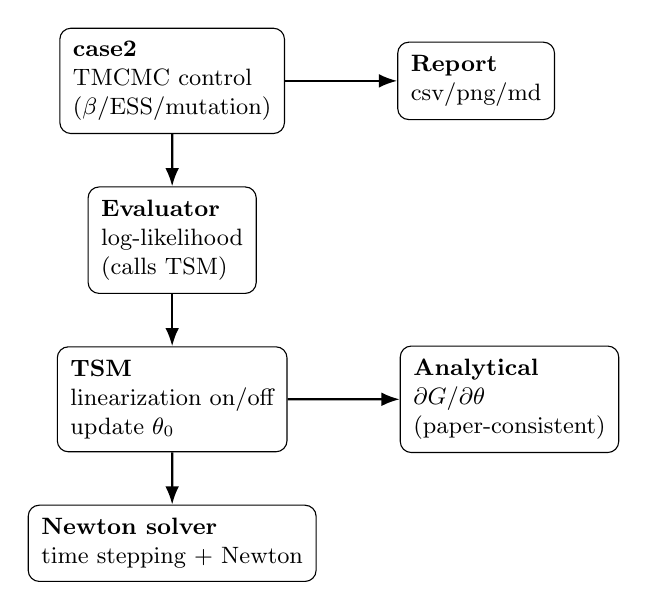
\begin{tikzpicture}[
  node/.style={draw,rounded corners,align=left,inner sep=5pt,font=\small},
  arrow/.style={-Latex,thick},
  scale=0.95, every node/.style={transform shape}
]
  \node[node] (case2) {\textbf{case2}\\TMCMC control\\($\beta$/ESS/mutation)};
  \node[node,below=7mm of case2] (eval) {\textbf{Evaluator}\\log-likelihood\\(calls TSM)};
  \node[node,below=7mm of eval] (tsm) {\textbf{TSM}\\linearization on/off\\update $\theta_0$};
  \node[node,below=7mm of tsm] (solver) {\textbf{Newton solver}\\time stepping + Newton};
  \node[node,right=15mm of tsm] (deriv) {\textbf{Analytical}\\$\partial G/\partial\theta$\\(paper-consistent)};
  \node[node,right=15mm of case2] (report) {\textbf{Report}\\csv/png/md};

  \draw[arrow] (case2) -- (eval);
  \draw[arrow] (eval) -- (tsm);
  \draw[arrow] (tsm) -- (solver);
  \draw[arrow] (tsm) -- (deriv);
  \draw[arrow] (case2) -- (report);
\end{tikzpicture}
\end{frame}

\begin{frame}{TMCMC essentials}
\begin{itemize}
  \item Tempering from prior ($\beta=0$) to posterior ($\beta=1$)
  \item Choose $\Delta\beta$ per stage based on target ESS (with min/max caps)
  \item Weight update $\rightarrow$ ESS $\rightarrow$ resample $\rightarrow$ mutation (MCMC) for mixing
\end{itemize}
\begin{alertblock}{Critical check}
Confirm \textbf{$\beta$ reaches 1.0} (log message like ``$\beta$ reached 1.0'').
\end{alertblock}
\end{frame}

\begin{frame}{TSM-ROM essentials (linearization management)}
\begin{block}{Local linearization}
\begin{equation}
x(\theta) \approx x(\theta_0) + \frac{\partial x}{\partial\theta}\Big|_{\theta_0}(\theta-\theta_0)
\end{equation}
\end{block}
\begin{itemize}
  \item Early stages: linearization OFF (robust exploration)
  \item Later stages: linearization ON (fast and accurate near MAP)
  \item Update point: \texttt{update\_linearization\_point($\theta_0$)} invalidates caches and recomputes
\end{itemize}
\end{frame}

\begin{frame}{When do we linearize? (concept)}
\centering
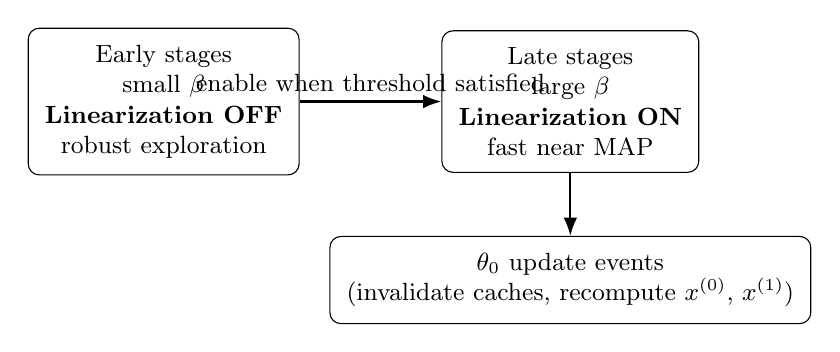
\begin{tikzpicture}[
  font=\small,
  arrow/.style={-Latex,thick},
  box/.style={draw,rounded corners,align=center,inner sep=6pt},
]
  \node[box] (early) {Early stages\\small $\beta$\\\textbf{Linearization OFF}\\robust exploration};
  \node[box,right=18mm of early] (late) {Late stages\\large $\beta$\\\textbf{Linearization ON}\\fast near MAP};
  \node[box,below=8mm of late] (upd) {$\theta_0$ update events\\(invalidate caches, recompute $x^{(0)}$, $x^{(1)}$)};
  \draw[arrow] (early) -- node[above]{enable when threshold satisfied} (late);
  \draw[arrow] (late) -- (upd);
\end{tikzpicture}
\vspace{2mm}
\begin{itemize}
  \item Enable linearization only after the posterior mass concentrates (avoid bias / instability).
  \item Track ROM error and $\|\Delta\theta_0\|$ to detect bad updates.
\end{itemize}
\end{frame}

\begin{frame}{Physical solver}
\begin{itemize}
  \item \texttt{run\_deterministic}: time integration with Newton solve per step
  \item \texttt{compute\_Q\_vector}, \texttt{compute\_Jacobian\_matrix}: residual and Jacobian
  \item Time-dependent antibiotics via \texttt{alpha\_schedule} (switch\_time/step/frac)
\end{itemize}
\end{frame}

\begin{frame}{Accuracy drivers}
\begin{itemize}
  \item \textbf{Largest}: likelihood definition ($\sigma_{\mathrm{obs}}$, variance model; Cov inclusion in Var)
  \item \textbf{Large}: ROM validity (ROM error, linearization update rules, analytical derivatives)
  \item \textbf{Medium}: numerical stabilization (dt, Newton tolerances, clipping/penalties)
  \item \textbf{Medium}: TMCMC settings (particles, stages, mutation steps)
\end{itemize}
\end{frame}

\begin{frame}{Performance drivers}
\begin{itemize}
  \item \textbf{Largest}: \texttt{BiofilmTSM\_Analytical.solve\_tsm()}
  \item \textbf{Largest}: \texttt{BiofilmNewtonSolver.run\_deterministic()} (Q/J + Newton)
  \item \textbf{Large}: sensitivity $x^{(1)}$ generation (esp. before linearization kicks in)
  \item \textbf{Medium}: TMCMC mechanics (resample/mutation/$\beta$ update)
\end{itemize}
\end{frame}

\begin{frame}{Reproducibility (audit artifacts)}
\begin{itemize}
  \item \texttt{config.json}: seeds and full configuration
  \item \texttt{likelihood\_meta\_*.json}: explicit likelihood definition
  \item \texttt{diagnostics\_tables/*.csv}: $\beta$, acceptance, ROM error, $\theta_0$ history
  \item \texttt{REPORT.md}: PASS/WARN/FAIL summary
\end{itemize}
\vspace{3mm}
\small
\textbf{One-command pipeline:}
\begin{quote}\small
\texttt{python tmcmc/run\_pipeline.py --mode paper --seed 123 --run-id paper\_M1\_seed123\_fixed --models M1 --lock-paper-conditions --use-paper-analytical}
\end{quote}
\textbf{Paper-fixed conditions:} \texttt{sigma\_obs=0.01}, \texttt{cov\_rel=0.005}
\end{frame}

\begin{frame}{Figure ideas}
\begin{itemize}
  \item $\beta$ schedule (per chain)
  \item ROM error at linearization updates (pre/post)
  \item $\|\Delta\theta_0\|$ history
  \item Posterior plots and MAP/MEAN fits
  \item Cost--accuracy tradeoff
\end{itemize}
\end{frame}

\begin{frame}{Example results (auto-picked best run)}
\small Best run id: \texttt{\BestRunId}. Figures are embedded only if present.
\vspace{2mm}
\begin{columns}[T,onlytextwidth]
  \column{0.5\textwidth}
  \IfFileExists{\BestRunFig{posterior_M1.png}}{
    \includegraphics[width=\linewidth]{\BestRunFig{posterior_M1.png}}
  }{\fbox{\parbox{\linewidth}{Missing: \texttt{posterior\_M1.png}}}}
  \column{0.5\textwidth}
  \IfFileExists{\BestRunFig{TSM_simulation_M1_MAP_fit_with_data.png}}{
    \includegraphics[width=\linewidth]{\BestRunFig{TSM_simulation_M1_MAP_fit_with_data.png}}
  }{\fbox{\parbox{\linewidth}{Missing: \texttt{MAP\_fit\_with\_data.png}}}}
\end{columns}
\end{frame}

\begin{frame}{Example diagnostics (ROM validity)}
\begin{columns}[T,onlytextwidth]
  \column{0.5\textwidth}
  \IfFileExists{\BestRunAsset{M1_rom_error.png}}{
    \includegraphics[width=\linewidth]{\BestRunAsset{M1_rom_error.png}}
  }{\fbox{\parbox{\linewidth}{Missing: \texttt{M1\_rom\_error.png}}}}
  \column{0.5\textwidth}
  \IfFileExists{\BestRunAsset{M1_theta0_step_norm.png}}{
    \includegraphics[width=\linewidth]{\BestRunAsset{M1_theta0_step_norm.png}}
  }{\fbox{\parbox{\linewidth}{Missing: \texttt{M1\_theta0\_step\_norm.png}}}}
\end{columns}
\end{frame}

\begin{frame}{Summary}
\begin{itemize}
  \item Pipeline: \texttt{run\_pipeline} $\rightarrow$ \texttt{case2} $\rightarrow$ \texttt{make\_report}
  \item Runtime dominated by \texttt{solve\_tsm} and Newton time stepping
  \item Audit essentials: \textbf{$\beta=1$ reached} and explicit likelihood definition
\end{itemize}
\end{frame}

\begin{frame}{PASS checklist (before claiming results)}
\begin{alertblock}{Minimum acceptance criteria}
\begin{itemize}
  \item $\beta$ reached 1.0 for all chains (posterior reached)
  \item \texttt{likelihood\_meta\_*.json} archived (variance model is explicit)
  \item No NaN/Inf in solver logs; diagnostics CSVs exist
  \item ROM validity monitored (ROM error + $\|\Delta\theta_0\|$ are stable)
\end{itemize}
\end{alertblock}
\end{frame}

\begin{frame}{References}
\footnotesize
\begin{thebibliography}{99}
\bibitem{Fritsch2025BayesianMicrofilms}
Fritsch, L., Geisler, H., Grashorn, J., Klempt, F., Soleimani, M., Broggi, M., Junker, P., Beer, M.
\textit{Bayesian updating of bacterial microfilms under hybrid uncertainties with a novel surrogate model}.
\texttt{tmcmc/Bayesian updating of bacterial microfilms under hybrid uncertainties with a novel surrogate model - Kopie.pdf}.

\bibitem{Klempt2025ContinuumBiofilm}
Klempt, F., Geisler, H., Soleimani, M., Junker, P.
\textit{A continuum multi-species biofilm model with a novel interaction scheme}. arXiv:2509.01274v1 (2025).
\texttt{tmcmc/biofilm\_simulation.pdf}.

\bibitem{JunkerBalzani2021ExtendedHamilton}
Junker, P., Balzani, D.
\textit{An extended Hamilton principle as unifying theory for coupled problems and dissipative microstructure evolution}.
Continuum Mechanics and Thermodynamics (2021). DOI: \texttt{10.1007/s00161-021-01017-z}.
\texttt{tmcmc/hamiltonian.pdf}.

\bibitem{Heine2025PeriImplant}
Heine, N. et al.
\textit{Influence of species composition and cultivation condition on peri-implant biofilm dysbiosis in vitro}.
Frontiers in Oral Health (2025). DOI: \texttt{10.3389/froh.2025.1649419}.
\texttt{tmcmc/Influence of species composition and cultivation condition on peri-implant biofilm dysbiosis in vitro.pdf}.
\end{thebibliography}
\end{frame}

\end{document}
